\documentclass[11pt]{article}
\usepackage[margin=1in]{geometry}
\usepackage{booktabs}
\usepackage{amsmath}
\usepackage{hyperref}
\usepackage{parskip}
\usepackage[expansion=false]{microtype}
\usepackage{xcolor}
\usepackage{mdframed}
\usepackage{enumitem}
\usepackage{graphicx}
\usepackage{tikz}

\definecolor{todocolor}{RGB}{220,240,255}
\definecolor{todoline}{RGB}{100,160,220}

\newmdenv[
  backgroundcolor=todocolor,
  linecolor=todoline,
  linewidth=1.5pt,
  innertopmargin=6pt,
  innerbottommargin=6pt,
  innerleftmargin=8pt,
  innerrightmargin=8pt,
  skipabove=8pt,
  skipbelow=8pt
]{todo}

\hypersetup{colorlinks=true, linkcolor=blue, urlcolor=blue}

\title{Caregiver Failed Extubation Rate and Patient Mortality:\\
\large Working Document --- June 2026}
\author{Zack Treisman}
\date{}

\begin{document}
\maketitle

\noindent This is a working document summarizing analyses completed to date and addressing questions raised by Andrew and Ryan. Blue boxes are remaining action items. All analyses use MIMIC-IV v3.1 (Beth Israel Deaconess Medical Center, 2008--2022). The primary outcome is \textbf{12-month mortality} throughout; all results from prior versions that used 12-month survival have been converted to the mortality framing for consistency with hospital and 30-day mortality secondary endpoints.

%% ──────────────────────────────────────────────────────
\section{Cohort and Data}

\subsection{Invasive vs.\ non-invasive ventilation}

There is an indicator variable in MIMIC-IV distinguishing invasive
(endotracheal) intubation from non-invasive ventilation (CPAP/BiPAP). I confirmed that the pipeline filters to \texttt{InvasiveVent} only. The other categoires are \texttt{SupplementalOxygen}, \texttt{NonInvasiveVent}, \texttt{HFNC}, \texttt{Tracheostomy}.

\subsection{Cohort sizes and covariate comparison}

\begin{table}[h!]
\centering
\begin{tabular}{lrr}
\toprule
Stage & N patients & Lost \\
\midrule
InvasiveVent $\geq$4h in MIMIC-IV v3.1 & 27,729 & \\
\quad of whom: explicit extubation documented & 18,958 & \\
\quad of whom: extubation inferred from vent record & 8,771 & \\
\addlinespace
\textit{Filters applied to both groups:} & & \\
\quad Died in hospital without extubation & & $-6{,}050$ \\
\quad Transitioned to tracheostomy & & $-1{,}523$ \\
\quad No computable ventilation duration & & $-8{,}068$ \\
\quad Incomplete covariates or non-ICU unit & & $-68$ \\
\midrule
\textbf{patient\_cohort} (last extubation per patient) & \textbf{12,662} & \\
\addlinespace
\quad Inferred events (no caregiver link) & & $-7{,}826$ \\
\quad Caregiver total volume $< 20$ or non-standard unit & & $-810$ \\
\midrule
\textbf{explicit\_extubations} (caregiver\_n $\geq$ 20) & \textbf{4,026} & \\
\quad Unique caregivers & 166 & \\
\quad ICU units & 8 & \\
\addlinespace
\quad Caregiver unit-specific volume $< 20$ & & $-600$ \\
\midrule
\textbf{analysis\_base} (primary analysis cohort) & \textbf{3,426} & \\
\quad CVICU & 1,435 & \\
\quad Medical (MICU + MICU/SICU) & 1,001 & \\
\quad Surgical/Trauma (SICU + TSICU) & 809 & \\
\quad Other units (descriptive only) & 181 & \\
\bottomrule
\end{tabular}
\caption{Cohort flow from all invasively ventilated patients in MIMIC-IV to the primary analysis cohort. The \texttt{patient\_cohort} ($N=12{,}662$) is used for descriptive analyses. The \texttt{explicit\_extubations} cohort ($N=4{,}026$) requires a genuine caregiver assignment and a caregiver total volume $\geq 20$. The \texttt{analysis\_base} ($N=3{,}426$) additionally requires caregiver unit-specific volume $\geq 20$, which is the denominator used to compute \texttt{caregiver\_fe\_rate}. See Table~\ref{tab:threshold} for the statistical rationale and
caregiver-count cost at each threshold.}
\label{tab:cohort_flow}
\end{table}

\begin{table}[h!]
\centering
\small
\begin{tabular}{lrrrr}
\toprule
 & $n \geq 5$ & $n \geq 10$ & $n \geq 20$ & $n \geq 32$ \\
\midrule
\textit{Statistical reliability (true FE rate = 5\%)} & & & & \\
\quad $P(\text{observe 0\% FE}) = 0.95^n$ & 77.4\% & 59.9\% & 35.8\% & 19.4\% \\
\quad $P(\text{observe} \geq 1 \text{ failure}) = 1 - 0.95^n$ & 22.6\% & 40.1\% & 64.2\% & \textbf{80.6\%} \\
\midrule
\textit{Eligible caregivers per unit (\texttt{caregiver\_n} $> 0$)} & & & & \\
\quad CVICU           & 141 & 136 & 102 & 71 \\
\quad MICU            & 107 &  87 &  47 & 33 \\
\quad TSICU           & 102 &  89 &  48 & 31 \\
\quad SICU            &  97 &  73 &  40 & 28 \\
\quad MICU/SICU       &  67 &  55 &  32 & 21 \\
\quad CCU             &  53 &  40 &  26 & 15 \\
\quad Neuro SICU      &  25 &  17 &   4 &  0 \\
\quad Neuro Intermed. &  19 &   9 &   1 &  0 \\
\quad Neuro Stepdown  &  10 &   1 &   0 &  0 \\
\bottomrule
\end{tabular}
\caption{Statistical reliability of the caregiver FE rate label and
caregiver retention at each unit-specific volume threshold. Top rows:
probability of observing zero failures (falsely appearing 0\% FE) vs.\
at least one failure for a caregiver whose true underlying rate is 5\%.
Bottom rows: number of eligible caregivers per unit at each threshold.
The $n \geq 32$ threshold achieves 80\% power to detect at least one
failure but eliminates the Neuro units and reduces the medical/surgical
groups by 30--40\%. The analysis uses $n \geq 20$ as a practical
compromise retaining all six primary units with $\geq 20$ caregivers each.
Neuro units are excluded from the primary MSM analysis regardless of threshold.}
\label{tab:threshold}
\end{table}

\begin{table}[h!]
\centering
\begin{tabular}{lrrr}
\toprule
 & All patients & \texttt{explicit\_extubations} & \texttt{analysis\_base}  \\
\midrule
N & 12,662 & 4,026 & 3,426 \\
Age, mean (SD) & 62.7 (16.2) & 63.1 (15.6) & 63.3 (15.6) \\
Female, \% & 40.7 & 38.0 & 38.0 \\
Charlson, mean (SD) & 5.57 (3.25) & 5.46 (3.23) & 5.46 (3.23)  \\
SOFA, mean (SD) & 6.91 (3.86) & 6.47 (3.52) & 6.34 (3.45) \\
Norepinephrine, mean (SD) & 0.17 (0.23) & 0.15 (0.19) & 0.14 (0.19)  \\
Vent hours, mean (SD) & 94.3 (134.1) & 64.3 (95.1) & 61.0 (91.8) \\
Medical-respiratory intubation, \% & 74.7 & 64.3 & 64.8 \\
Circulatory primary diagnosis, \% & 32.9 & 42.6 & 42.8 \\
12-month mortality, \% & 45.2 & 32.1 & 30.0 \\
Hospital mortality, \% & 27.3 & 12.0 & 11.9 \\
\bottomrule
\end{tabular}
\caption{Comparison of the full patient cohort vs.\ \texttt{explicit\_extubations}
(explicit events with \texttt{caregiver\_n} $\geq 20$, standard ICU unit) vs.\ the primary analysis cohort \texttt{analysis\_base} (additional \texttt{caregiver\_unit\_n} $\geq 20$). The analytical cohorts are systematically less sick than the full \texttt{patient\_cohort}: lower SOFA, shorter ventilation, lower mortality, reflecting selection toward patients with better-documented, shorter ICU stays. The two analytical cohorts are similar to each other; the unit-volume threshold
($-600$ patients) causes minimal further selection.}
\label{tab:cohort_comparison}
\end{table}

Tables \ref{tab:cohort_flow}--\ref{tab:cohort_comparison} summarize cohort flow and characteristics. The primary analysis cohort (\texttt{analysis\_base}) includes 3,426 patients with explicit extubation events, caregiver volume $\geq 20$ at the unit level, and standard ICU unit labels. The \texttt{patient\_cohort} ($N=12{,}662$) is used for descriptive analyses of the full population of invasively ventilated patients with extubation events, including those without a caregiver link and those in non-ICU units.

When the extubation event is inferred from the ventilation record rather than explicitly documented, there is no caregiver link and the patient is excluded from the primary analysis. These patients are included in the \texttt{patient\_cohort} for descriptive purposes but not in any caregiver-level analyses. An additional complication with these patients is that vent duration is highly uncertain. Attempts to impute caregiver assignment for inferred events have not yet yielded a reliable method; this remains an open question for future work.

\noindent A note on caregiver attribution: \texttt{caregiver\_id} in MIMIC-IV records the \emph{documenting} user, not necessarily the provider who performed the extubation. This is a known limitation of the dataset.

\noindent \textbf{Non-ICU units excluded:} Four unit labels were identified as non-standard settings and excluded from the primary analysis: PACU ($N=19$), generic ``ICU'' ($N=12$), Surgery/Vascular/Intermediate ($N=76$, $\approx$50\% COVID diagnoses, vent hours $>$220h, likely COVID-era overflow ward), and Medicine ($N=11$). These patients are retained in patient\_cohort but not in the primary analysis cohort.

\begin{todo} 
  \textbf{TODO: CONSORT diagram:} Create a flow diagram visualizing the cohort flow from all invasively ventilated patients to the final analysis cohort, with counts and reasons for exclusion at each step.
\end{todo}

\subsection{Terminal extubation}
\label{sec:terminal}

The current analysis uses death within 3 days of extubation as the criterion for a likely comfort extubation, flagging 175 patients (4.3\% of the analytical cohort). A sensitivity analysis excluding these cases is reported in Section~\ref{sec:comfort}.

\noindent \textbf{Andrew's note on code status:} Death within 3 days is a rough proxy --- it captures patients extubated with survival intent who had unexpected deterioration, not only those extubated as comfort care. A more specific marker would be a documented change in code status (DNR/DNI order) in the 24--48h preceding extubation, which is available in MIMIC-IV \texttt{chartevents}. This query has not yet been run; it is a priority for the next revision.

\begin{todo}
  \textbf{TODO: code status query:} Run a query to identify patients with a documented change in code status to DNR/DNI in the 24--48h preceding extubation. Use this to refine the comfort extubation sensitivity analysis.
\end{todo}



%% ──────────────────────────────────────────────────────
\section{ICU Unit Breakdown}

\begin{figure}[h!]
\centering
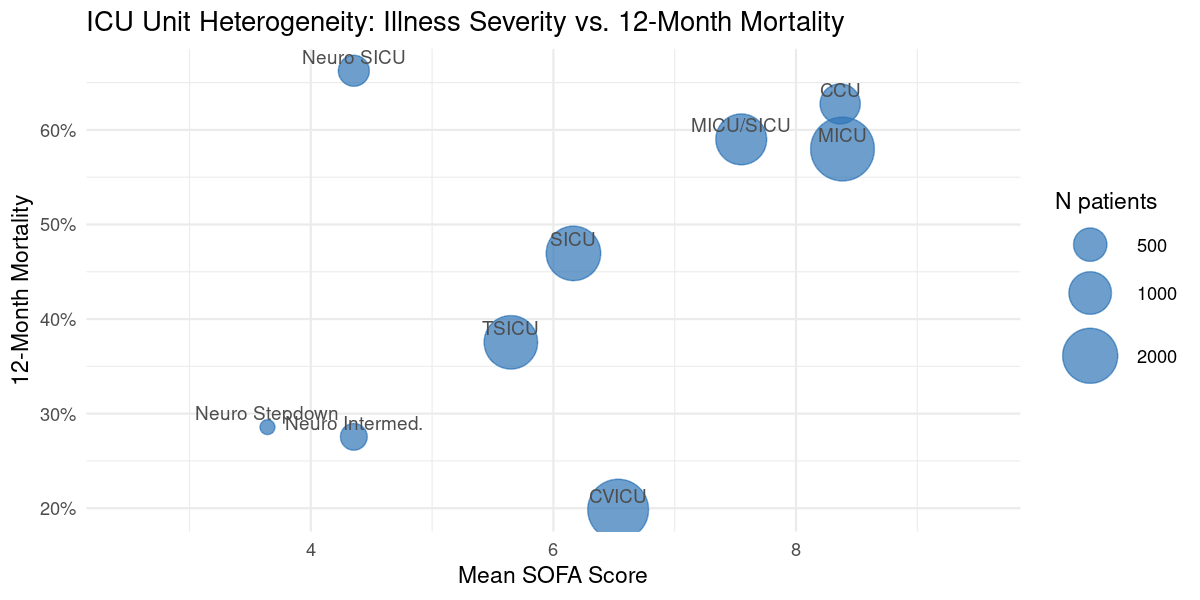
\includegraphics[width=0.9\textwidth]{../figures/unit_sofa_mortality.png}
\caption{ICU unit heterogeneity: mean SOFA score vs.\ 12-month mortality.
Bubble size proportional to patient count.}
\label{fig:unit_sofa}
\end{figure}


\begin{table}[h!]
\centering
\small
\begin{tabular}{lrrrrrr}
\toprule
Unit & N & Age & SOFA & Charlson & Vent h & 12-mo mortality \\
 & & mean (SD) & mean (SD) & mean (SD) & median [IQR] & \% \\
\midrule
CVICU        & 2,585 & 66.5 (12.5) & 6.5 (3.3) & 5.4 (2.9) & 14 [6--45]   & 19.8 \\
TSICU        & 1,854 & 58.7 (19.2) & 5.7 (3.5) & 4.3 (3.3) & 44 [15--122] & 37.5 \\
SICU         & 1,947 & 62.7 (15.9) & 6.2 (4.0) & 5.6 (3.0) & 42 [17--123] & 46.9 \\
MICU         & 2,915 & 61.3 (16.5) & 8.4 (4.0) & 6.0 (3.3) & 64 [23--154] & 58.0 \\
MICU/SICU    & 1,622 & 61.8 (16.9) & 7.6 (3.8) & 6.1 (3.5) & 54 [18--142] & 59.0 \\
CCU          & 851   & 67.6 (13.9) & 8.4 (3.5) & 7.0 (2.9) & 50 [20--114] & 62.7 \\
Neuro SICU   & 403   & 64.7 (16.3) & 4.4 (3.0) & 5.7 (3.2) & 33 [15--82]  & 66.3 \\
Neuro Intermed. & 265 & 58.9 (17.0) & 4.4 (2.9) & 4.9 (3.0) & 35 [17--81] & 27.5 \\
Neuro Stepdown  & 98  & 58.6 (16.3) & 3.6 (2.2) & 4.4 (3.0) & 25 [12--66] & 28.6 \\
\bottomrule
\end{tabular}
\caption{Patient profiles by ICU unit (\texttt{patient\_cohort}, N=12,662; explicit + inferred events). Units ordered by 12-month mortality (ascending). Neuro units listed last. See Table~\ref{tab:caregivers} for unit-specific FE rates in the analytical cohort. There is no separate CTICU label in MIMIC-IV. The cardiac surgery recovery unit appears exclusively as ``Cardiac Vascular Intensive Care Unit (CVICU).''}
\label{tab:units}
\end{table}


\subsection{Unit clinical profiles}

The eight recognized ICU units in the analytical cohort fall into four
clinically distinct groups:

\textbf{Cardiac Vascular ICU (CVICU, $N=2{,}585$ in patient\_cohort).} Oldest patients (mean 66.5y), 84\% circulatory diagnoses, short ventilation (55h mean), lowest FE rate (1.8\%), best outcomes (13.7\% 12-month mortality in \texttt{analysis\_base}). Extubation is a near-routine step in surgical recovery.
\textbf{Andrew's note on CVICU vs.\ CTICU:} There is no separate
``Cardiothoracic ICU'' label in MIMIC-IV; all cardiac surgery and cardiac medical admissions appear under the single CVICU label. Among CVICU patients in the analytical cohort, 84.2\% have a circulatory primary ICD chapter and 45.2\% have medical-non-respiratory intubation type (a proxy for cardiac surgery recovery). The remainder are likely post-MI and other non-surgical cardiac events.

\textbf{Medical critical care (MICU + MICU/SICU, $N=4{,}537$).} Highest SOFA (8.4 and 7.6), longest ventilation (118h and 111h), 88\%+ medical-respiratory intubation. MICU dominated by infectious (28\%) and respiratory (20\%) diagnoses. 12-month mortality approximately 48--56\%.

\textbf{Surgical and trauma (SICU + TSICU, $N=3{,}801$).} TSICU: youngest (58.7y), lowest Charlson (4.3), 46\% injury/poisoning diagnoses. SICU: more heterogeneous (17.9\% digestive, 15.5\% injury, 11.2\% neoplasms).

\textbf{Cardiac care (CCU, $N=851$).} Oldest alongside CVICU (67.6y), highest Charlson (7.0), 64\% circulatory diagnoses. 56.2\% 12-month mortality despite ``only'' 40.8\% hospital mortality --- substantial post-discharge mortality. Excluded from the primary MSM analysis due to insufficient caregiver volume with the $\geq 20$ unit-extubation threshold (2 eligible caregivers).

\textbf{Neuro units ($N=766$).} \textbf{Andrew's note:} The ``Neuro Surgical ICU (Neuro SICU)'' label in MIMIC-IV is used for patients with primary neurological diagnoses including both neurosurgical and medical neurology admissions (13.4\% neurologic, 18.1\% injury/poisoning, 51.4\% circulatory --- the last group perhaps representing aneurysm and AVM cases). It is not a pure neurosurgical unit. Neuro Intermediate and Stepdown have lower mortality(28\% and 25\%) and are step-down rather than full ICU settings; all three are excluded from the primary analysis due to small caregiver counts.

%% ────────────────────────────────────────────────────
\section{Caregiver Profiles}

Table~\ref{tab:caregiver_flow} summarizes the caregiver cohort flow. Of
131 unique caregivers in the primary analysis cohort, 207 caregiver--unit
group assignments exist (CVICU + Medical + Surgical/Trauma = 102 + 52 + 53),
meaning 76 caregivers provide care across multiple primary analysis groups
and are counted independently within each group with their unit-specific
FE rate.

\begin{table}[h!]
\centering
\begin{tabular}{lrr}
\toprule
Stage & N caregivers & Lost \\
\midrule
\textbf{Caregivers in \texttt{patient\_cohort}} & \textbf{570} & \\
\quad (all have explicit events; inferred events carry no caregiver link) & & \\
\addlinespace
\quad Total extubation volume $< 20$ (\texttt{caregiver\_n} $< 20$) & & $-404$ \\
\midrule
\textbf{Caregivers with volume $\geq 20$} & \textbf{166} & \\
\addlinespace
\quad Unit-specific volume $< 20$ in all units & & $-32$ \\
\midrule
\textbf{Caregivers in \texttt{analysis\_base}} (\texttt{caregiver\_unit\_n} $\geq 20$) & \textbf{134} & \\
\addlinespace
\quad In ``Other'' ICU units only (CCU, Neuro, non-standard) & & $-3$ \\
\midrule
\textbf{Caregivers in primary analysis groups} & \textbf{131} & \\
\quad CVICU (unit-specific) & 102 & \\
\quad Medical (MICU + MICU/SICU, unit-specific) & 52 & \\
\quad Surgical/Trauma (SICU + TSICU, unit-specific) & 53 & \\
\addlinespace
\quad \textit{Total caregiver--unit assignments} & \textit{207} & \\
\bottomrule
\end{tabular}
\caption{Caregiver cohort flow. The three per-group caregiver counts
(102 + 52 + 53 = 207) exceed the 131 unique caregivers because 76
caregivers work across multiple primary analysis groups and are counted
independently in each with their unit-specific FE rate.
Caregiver profiles by primary unit are shown in Table~\ref{tab:caregivers}.}
\label{tab:caregiver_flow}
\end{table}

\begin{table}[h!]
\centering
\small
\begin{tabular}{lrrrrrr}
\toprule
 & CVICU & MICU & TSICU & SICU & MICU/SICU & CCU \\
\midrule
N caregivers & 79 & 26 & 13 & 6 & 7 & 3 \\
\addlinespace
\textit{FE rate (unit-specific)} & & & & & & \\
\quad Median & 1.4\% & 4.5\% & 7.3\% & 2.6\% & 4.8\% & 0\% \\
\quad IQR & 0--3.6\% & 3.2--7.7\% & 5.6--7.4\% & 0.5--3.2\% & 1.6--7.7\% & 0--2.4\% \\
\quad Max & 11.1\% & 12.8\% & 16.0\% & 4.2\% & 10.6\% & 4.8\% \\
\addlinespace
\textit{Volume (total extubations)} & & & & & & \\
\quad Median & 73 & 278 & 42 & 128 & 32 & 24 \\
\quad IQR & 39--158 & 48--480 & 34--59 & 33--232 & 24--228 & 24--24 \\
\quad Max & 713 & 983 & 75 & 387 & 519 & 25 \\
\addlinespace
\textit{Patients in analytical sample} & & & & & & \\
\quad Median & 11 & 32 & 6 & 20 & 7 & 6 \\
\addlinespace
12-mo mortality, mean & 13.8\% & 39.6\% & 23.5\% & 34.6\% & 42.1\% & 58.3\% \\
\bottomrule
\end{tabular}
\caption{Caregiver profiles by primary ICU unit (\texttt{caregiver\_unit\_n} $\geq 20$, consistent with \texttt{analysis\_base}). Volume = total explicit extubation events in MIMIC-IV. CVICU has the largest number of eligible caregivers (79) despite lower individual volumes, reflecting a large cardiac surgery program. Median FE rate is 1.4\% for CVICU caregivers; most with 0\% rate are low-volume providers (see Section~\ref{sec:vol_confound}). MICU caregivers have the highest volume (median 278). CCU has only 3 caregivers meeting the threshold and is excluded from the primary MSM analysis.}
\label{tab:caregivers}
\end{table}

\begin{figure}[h!]
\centering
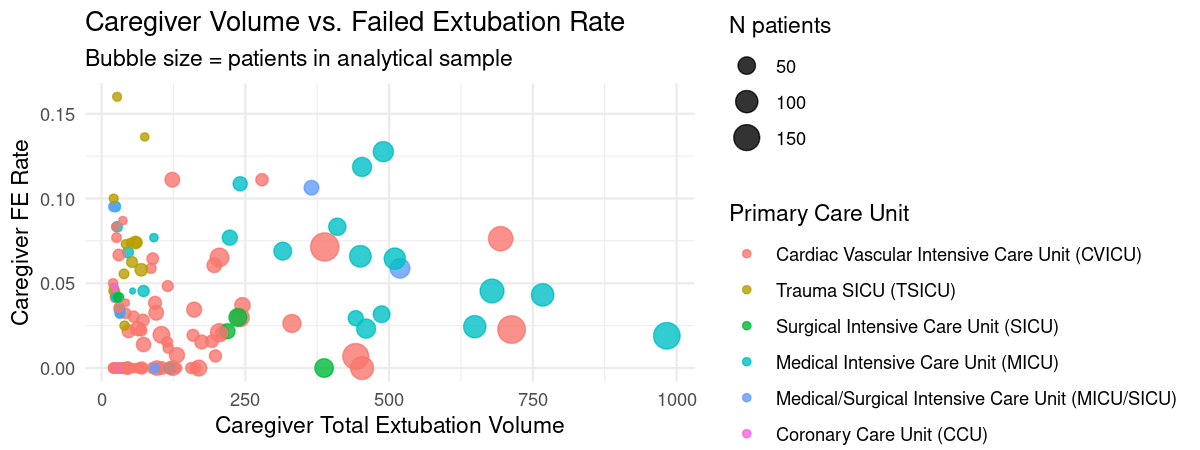
\includegraphics[width=\textwidth]{../figures/caregiver_vol_fe.png}
\caption{Caregiver total extubation volume vs.\ failed extubation rate.
Bubble size = patients in analytical sample.}
\label{fig:caregiver_vol_fe}
\end{figure}


%%
\section{Causal Analysis: Continuous Treatment MSM}
\label{sec:msm}

\subsection{Why we moved away from binary PSM}

The original analysis compared patients of top-quartile FE rate caregivers
(Q4) to bottom-quartile (Q1) caregivers. Andrew's review identified two
fundamental problems.

\textbf{The 0\%-FE stratum is driven by low volume.} In CVICU, the bottom
quartile consists entirely of caregivers who have had zero failed extubations
in their career (Q25 = 0\% at this unit). A characterization analysis
(Figure~\ref{fig:cvicu_strata}) reveals that this group is dominated by
\emph{low-volume} providers who have not accumulated enough extubations to
have had a failure yet. Among the 73 CVICU caregivers with a 0\% FE rate,
the median number of patients in the analytical sample is just 4 [IQR 2--6].
By contrast, providers with non-zero FE rates have median analytical-sample
volumes of 16--22 patients. The probability of observing zero failures by
chance (assuming a true underlying rate of 5\%) is $(0.95)^4 \approx 81\%$
with four observations. The 0\%-FE label is largely statistical noise for
these low-volume providers.
\label{sec:vol_confound}

\textbf{The propensity score has a weak conceptual basis here.} The
propensity score models $P(\text{assigned to high-FE caregiver} \mid
\text{patient covariates})$. As Andrew correctly noted, within an ICU,
patient-to-caregiver assignment is largely determined by staffing rosters,
not patient characteristics. Our analysis confirms this empirically: patient
covariates explain only 4--7\% of variance in caregiver FE rate in all three
unit groups (denominator $R^2 = 0.057$, $0.042$, $0.069$ for CVICU, Medical,
and Surgical/Trauma). The IPW weights are therefore close to 1 for most
patients, meaning the weighting is performing almost no confound correction.
This is consistent with near-random assignment.

\subsection{Method: stabilized density weights}

We replaced the binary PSM with a marginal structural model (MSM) for
continuous treatment (Robins et al.\ 2000; Hern{\'a}n \& Robins 2020,
\S12). The exposure is \texttt{caregiver\_fe\_rate} as a continuous variable;
all patients are included regardless of their caregiver's quartile. Stabilized
Hirano--Imbens density weights are:
\[
sw_i = \frac{f(T_i)}{f(T_i \mid X_i)}
\]
where $T = \texttt{caregiver\_fe\_rate}$, $X$ = patient covariates (age, sex,
Charlson, SOFA, norepinephrine, ventilation hours, intubation type, 21
CCSR diagnosis flags), and $f$ denotes a probability density function (PDF).
$f(T_i)$ is the \emph{marginal} density of the treatment evaluated at patient
$i$'s observed FE rate; $f(T_i \mid X_i)$ is the \emph{conditional} density
of treatment given patient covariates. Both are estimated as normal densities
from OLS: fitting $T_i = \alpha + X_i\beta + \varepsilon_i$ gives conditional
fitted values $\hat{T}_i$ and residual variance $\hat{\sigma}^2_{T|X}$, so
\[
f(T_i \mid X_i) = \frac{\phi\!\left(\dfrac{T_i - \hat{T}_i}{\hat{\sigma}_{T|X}}\right)}{\hat{\sigma}_{T|X}},
\qquad
f(T_i) = \frac{\phi\!\left(\dfrac{T_i - \bar{T}}{\hat{\sigma}_T}\right)}{\hat{\sigma}_T},
\]
where $\phi$ is the standard normal PDF and $\bar{T}$, $\hat{\sigma}_T$ are
the marginal mean and standard deviation of $T$. The ratio upweights patients
whose observed FE rate was unlikely given their covariates and downweights
those for whom it was expected, recreating a pseudo-population in which
covariates are balanced across FE rate levels. Weights are trimmed at the
99th percentile.
Primary inference uses cluster-robust standard errors by
\texttt{caregiver\_id}. The effect size is reported as the odds ratio per
5 percentage-point increase in caregiver FE rate (approximately the CVICU
IQR).

\begin{figure}[h!]
\centering
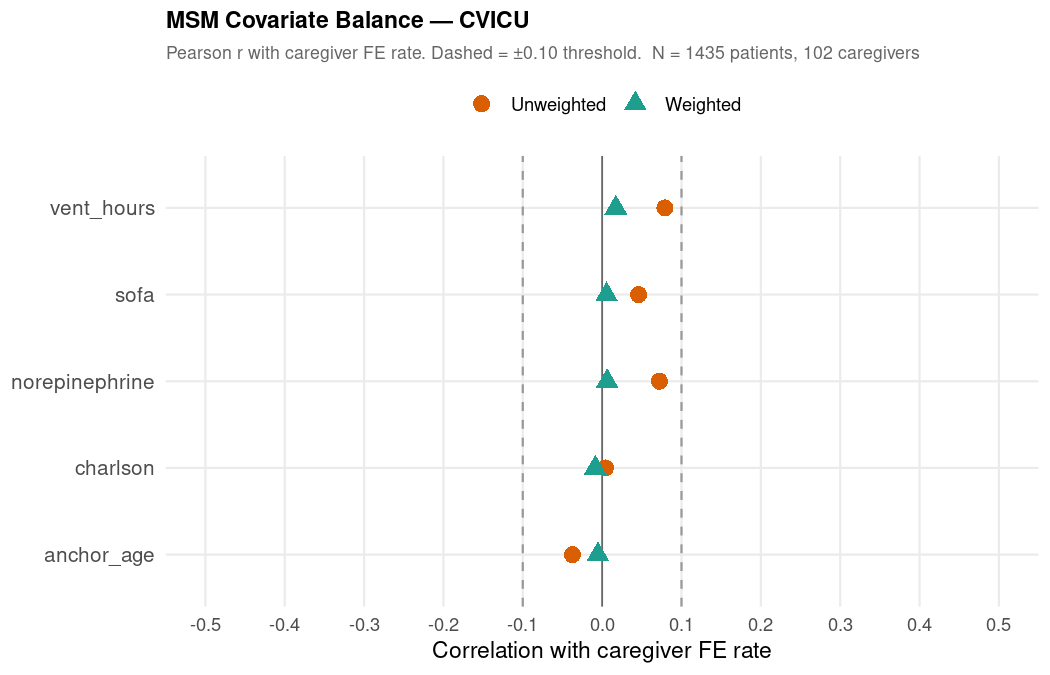
\includegraphics[width=0.75\textwidth]{../figures/msm_balance_cvicu.png}
\caption{MSM covariate balance --- CVICU. Pearson correlation of each
covariate with caregiver FE rate before (orange) and after (teal) IPW
weighting. Dashed lines = $\pm 0.10$ threshold. All covariates fall within
the threshold after weighting.}
\label{fig:msm_balance}
\end{figure}

\begin{figure}[h!]
\centering
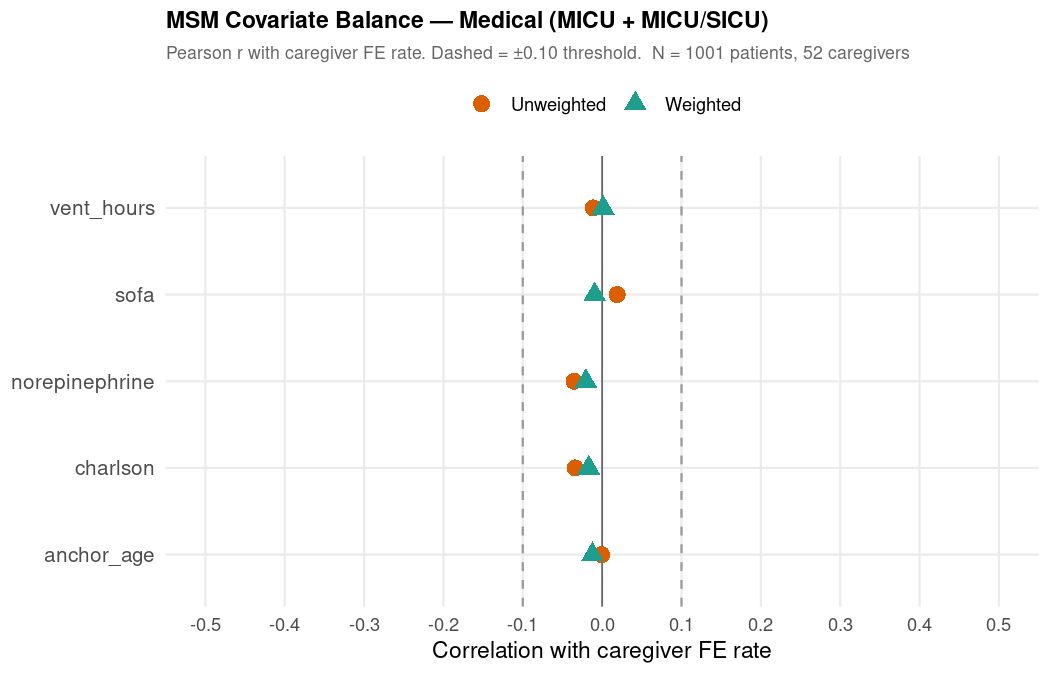
\includegraphics[width=0.75\textwidth]{../figures/msm_balance_medical__micu___micu_sicu_.png}
\caption{MSM covariate balance --- Medical (MICU + MICU/SICU). Pearson
correlation of each covariate with caregiver FE rate before (orange) and
after (teal) IPW weighting. Dashed lines = $\pm 0.10$ threshold.}
\label{fig:msm_balance_medical}
\end{figure}

\begin{figure}[h!]
\centering
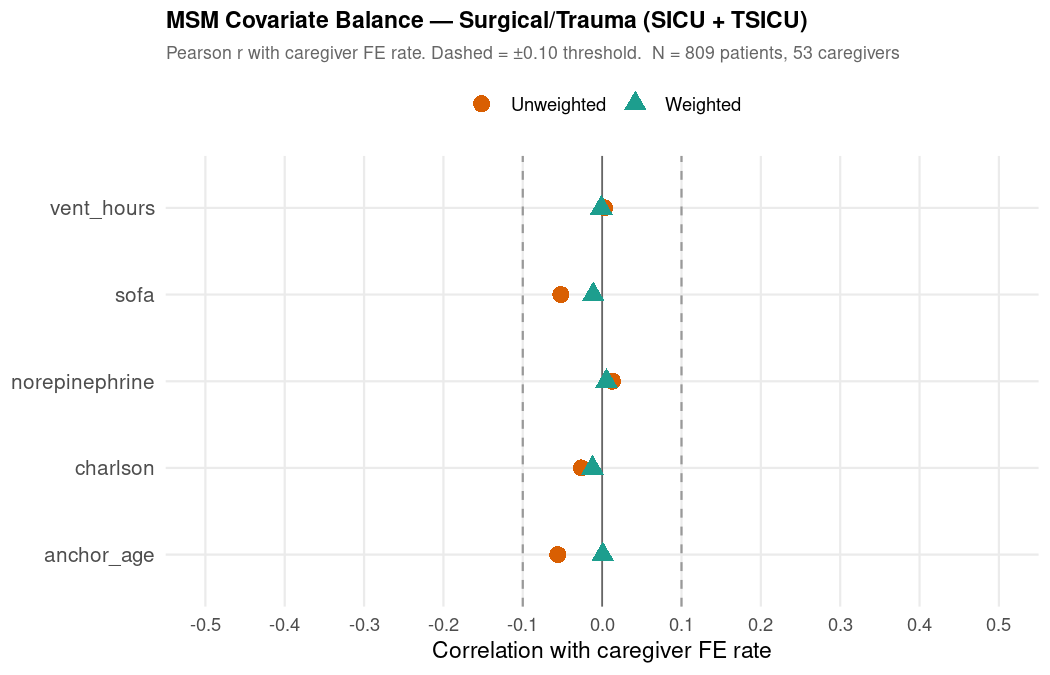
\includegraphics[width=0.75\textwidth]{../figures/msm_balance_surgical_trauma__sicu___tsicu_.png}
\caption{MSM covariate balance --- Surgical/Trauma (SICU + TSICU). Pearson
correlation of each covariate with caregiver FE rate before (orange) and
after (teal) IPW weighting. Dashed lines = $\pm 0.10$ threshold.}
\label{fig:msm_balance_surgical}
\end{figure}

\subsection{Results}

\begin{table}[h!]
\centering
\begin{tabular}{lrrrrrr}
\toprule
Group & N & Caregivers & Denom $R^2$ & OR per 5pp & 95\% CI & $p$ \\
\midrule
CVICU           & 1,435 & 102 & 0.057 & 1.432 & 0.931--2.200 & 0.102 \\
Medical         & 1,001 &  52 & 0.042 & 0.898 & 0.750--1.074 & 0.239 \\
Surgical/Trauma &   809 &  53 & 0.069 & 0.893 & 0.627--1.270 & 0.529 \\
\bottomrule
\end{tabular}
\caption{MSM results by unit group. Outcome: 12-month mortality. OR $>1$
indicates higher mortality for patients of higher-FE-rate caregivers. Denom
$R^2$ = variance in caregiver FE rate explained by patient covariates in the
denominator model; low values confirm near-random caregiver assignment.
Cluster-robust SEs by \texttt{caregiver\_id}.}
\label{tab:msm}
\end{table}

\begin{figure}[h!]
\centering
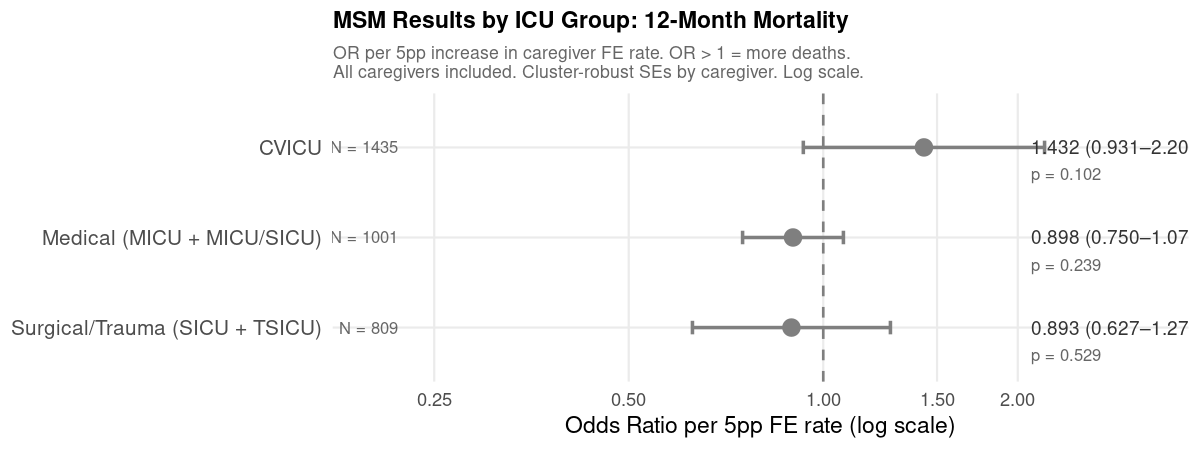
\includegraphics[width=0.8\textwidth]{../figures/msm_forest.png}
\caption{MSM results by ICU group: 12-month mortality odds ratio per 5
percentage-point increase in caregiver FE rate. OR $>1$ = more deaths with
higher FE rate. All groups are null ($p > 0.05$). Cluster-robust SEs by
caregiver.}
\label{fig:msm_forest}
\end{figure}

\noindent The CVICU point estimate (OR = 1.432) is directionally consistent
with the prior PSM finding (OR = 1.72 on the mortality scale), but does not
reach significance ($p = 0.102$). The denominator $R^2 = 0.057$ confirms that
patient covariates explain very little of caregiver FE rate variance, and the
effective sample size after weighting (1,392 of 1,435) shows the weights are
barely adjusting for confounding. Medical and Surgical/Trauma are null across
all methods.

\subsection{Secondary outcomes}

\begin{table}[h!]
\centering
\begin{tabular}{lrrrr}
\toprule
Group & Hosp.\ mortality OR & $p$ & 30-day mortality OR & $p$ \\
\midrule
CVICU & 1.408 (0.712--2.783) & 0.325 & 2.144 (0.788--5.829) & 0.135 \\
Medical & 1.120 (0.917--1.367) & 0.267 & 1.029 (0.807--1.313) & 0.817 \\
Surgical/Trauma & 0.856 (0.530--1.381) & 0.523 & 0.960 (0.636--1.447) & 0.844 \\
\bottomrule
\end{tabular}
\caption{Secondary mortality outcomes by ICU group. OR $>1$ = more deaths
with higher FE rate. All three mortality endpoints are now in the same
direction (OR $>1$ = worse); CVICU shows a consistent positive direction
across all three endpoints but does not reach significance at any. The
Surgical/Trauma 30-day signal seen in the prior PSM analysis does not
survive in the MSM.}
\label{tab:secondary}
\end{table}

\begin{figure}[h!]
\centering
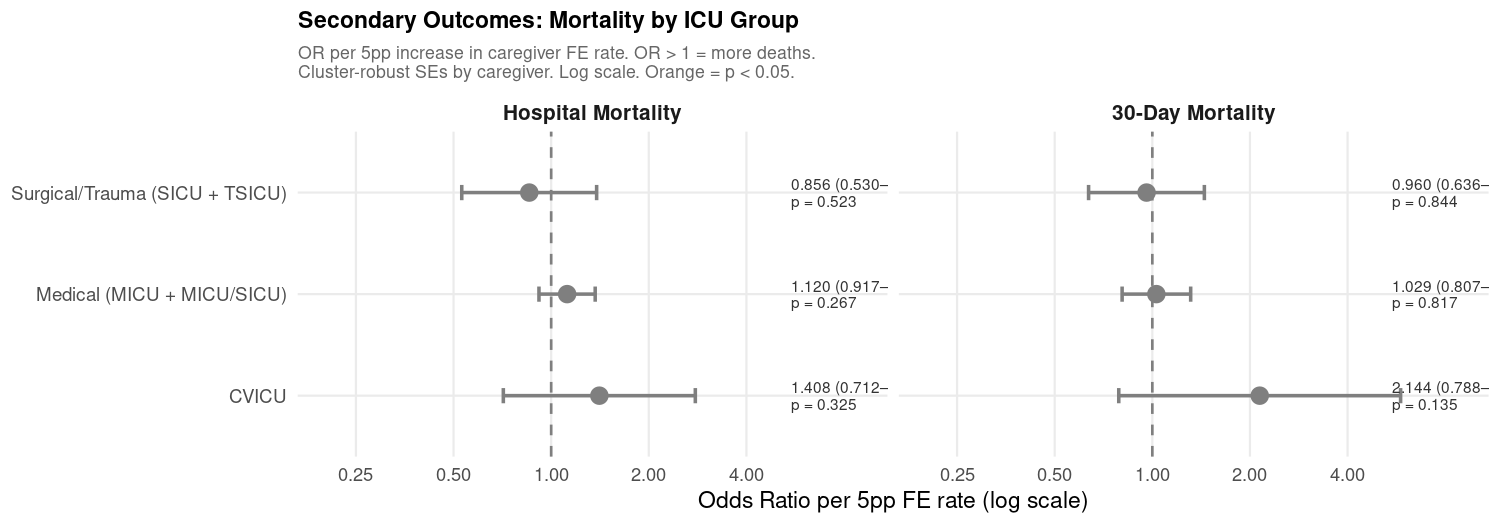
\includegraphics[width=0.8\textwidth]{../figures/msm_secondary_forest.png}
\caption{MSM secondary outcomes by ICU group: hospital and 30-day mortality.
OR $>1$ = more deaths with higher FE rate. All results are non-significant.}
\label{fig:msm_secondary_forest}
\end{figure}

\subsection{Comfort extubation sensitivity}
\label{sec:comfort}

Excluding likely comfort extubations (in-hospital death within 3 days;
$N = 10$ in CVICU, 0.7\%):

\begin{center}
\begin{tabular}{lrr}
\toprule
& MSM OR per 5pp & $p$ \\
\midrule
CVICU (all) & 1.432 & 0.102 \\
CVICU (comfort excluded) & 1.398 & 0.122 \\
\bottomrule
\end{tabular}
\end{center}

\noindent The CVICU direction is stable and the result is not driven by
comfort-care confounding.

\subsection{Volume confounding and the 0\%-FE stratum}
\label{sec:vol_confound_detail}

The caregiver characterization analysis (Table~\ref{tab:cvicu_strata})
explains why the 0\%-FE stratum shows better patient outcomes.

\begin{table}[h!]
\centering
\small
\begin{tabular}{lrrrrrr}
\toprule
FE rate stratum & N (pts) & N (caregivers) & Med vol & Max vol & Vent h (med) & Mortality \\
\midrule
0\% (exact) & 313 & 36 & 6 [4--10] & 45 & 8 [5--19] & 9.9\% \\
$>$0--median (1.96\%) & 569 & 22 & 16 [9--26] & 149 & 6 [4--19] & 13.7\% \\
median--Q75 (2.99\%) & 273 & 14 & 16 [12--22] & 56 & 12 [5--37] & 15.8\% \\
$>$Q75 & 280 & 30 & 8 [4--12] & 29 & 15 [5--36] & 15.7\% \\
\bottomrule
\end{tabular}
\caption{CVICU patient and caregiver characteristics by FE rate stratum
(\texttt{analysis\_base}, \texttt{caregiver\_unit\_n} $\geq 20$). Med vol = median patients in
analytical sample per caregiver [IQR]. The 0\%-FE stratum has the lowest
caregiver volumes and the shortest ventilation times --- both consistent with
a simpler case mix --- rather than any identifiable superiority in extubation
skill. SOFA, Charlson, and age are similar across all strata.}
\label{tab:cvicu_strata}
\end{table}

\noindent The 0\%-FE caregivers have median volume of 6 patients [IQR 4--10]
in the analytical sample, and their patients have shorter ventilation times
(8h median) than all other strata. This profile is consistent with occasional-coverage providers seeing
straightforward post-surgical cases who are easy to extubate. The caregiver
volume and case mix, not the FE rate per se, likely explain the mortality
difference in this stratum.

\begin{figure}[h!]
\centering
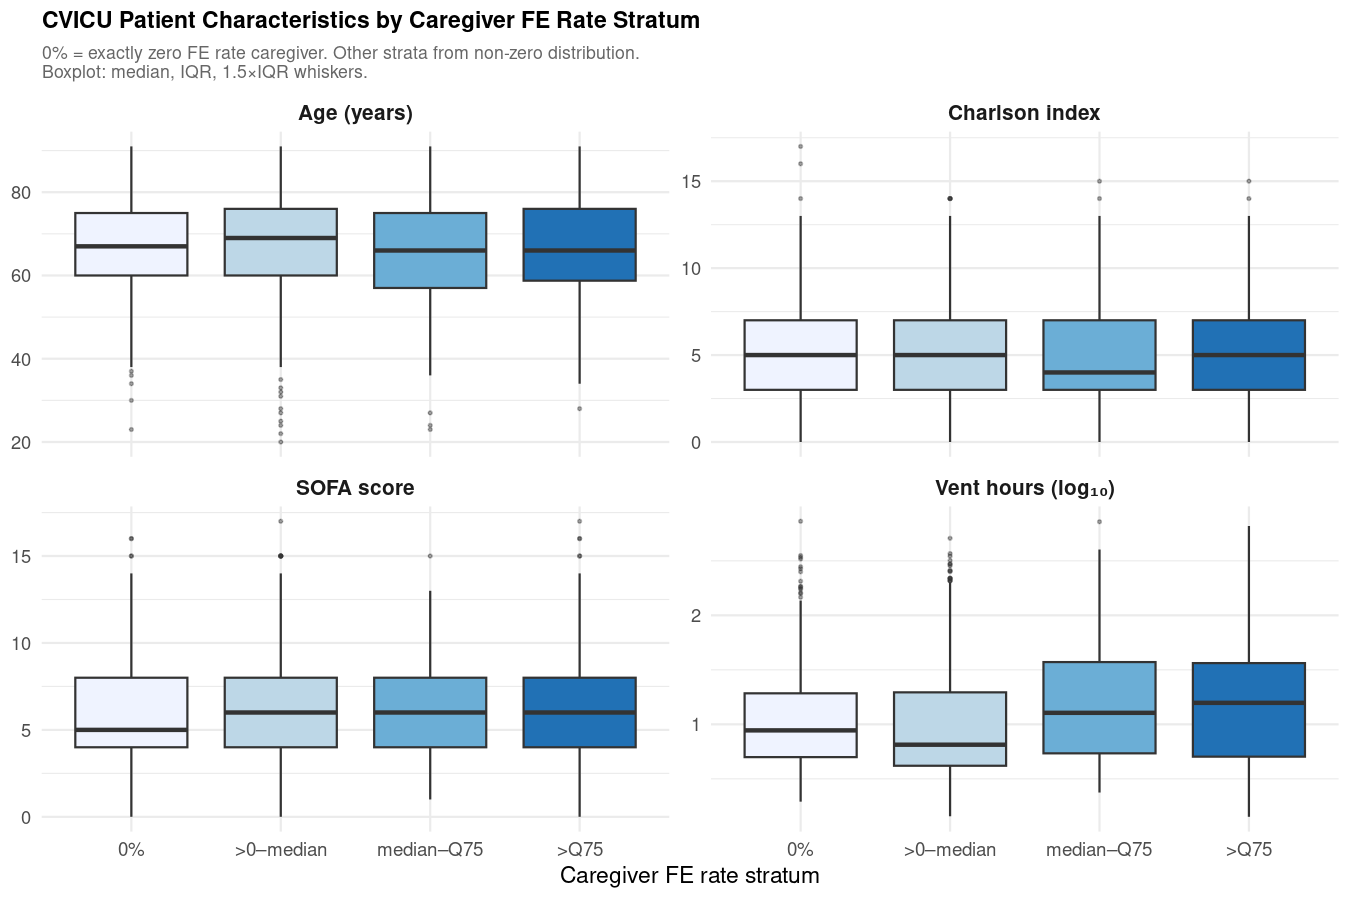
\includegraphics[width=0.85\textwidth]{../figures/cvicu_strata_covariates.png}
\caption{CVICU patient characteristics by caregiver FE rate stratum. SOFA,
age, and Charlson are similar across strata. Ventilation hours increase
monotonically with FE rate, consistent with higher FE rate caregivers
managing more complex, longer-ventilated patients. Log scale on vent hours.}
\label{fig:cvicu_strata}
\end{figure}

\subsection{Caregiver-level partial correlations}

At the caregiver level (one observation per caregiver, outcome = mean
12-month patient mortality), the partial correlation between FE rate and
mortality controlling for caregiver volume is:

\begin{center}
\begin{tabular}{lrrr}
\toprule
Cohort & N caregivers & $r$ (FE rate $\sim$ mortality) & $p$ \\
\midrule
analysis\_base (caregiver\_unit\_n $\geq 20$) & 134 & $+0.216$ & 0.012 \\
$+$ analytic patients $\geq 10$ & 70 & $+0.432$ & $<0.001$ \\
$+$ analytic patients $\geq 20$ & 42 & $+0.485$ & 0.001 \\
\bottomrule
\end{tabular}
\end{center}

\noindent The positive sign confirms the direction: higher FE rate caregivers
have patients with worse mortality, controlling for caregiver volume. The
association strengthens when restricted to caregivers with larger analytical
samples, suggesting it is not noise from small denominators. Volume also
carries independent signal when controlling for FE rate ($r = +0.282$,
$p = 0.001$).

\noindent The CVICU unit-stratified partial correlation is $r = +0.261$,
$p = 0.021$ ($N = 79$ caregivers) --- again specific to CVICU, consistent
with all patient-level analyses.

\section{Functional form: mortality ceiling}

Fitting $P(\text{mortality}) = m_{\max}\,(1 - e^{-k \cdot \text{FE rate}})$
at the caregiver level ($N = 90$ caregivers with FE rate $> 0$). This is
reparametrized from the equivalent survival floor form: $m_{\max} = 1 - b$
where $b$ is the survival floor. The mortality ceiling $m_{\max}$ represents
the maximum achievable 12-month mortality as FE rate $\to \infty$ ---
equivalently, the fraction of outcomes potentially sensitive to caregiver
extubation practice.

\begin{center}
\begin{tabular}{lrr}
\toprule
Parameter & Estimate & 95\% CI \\
\midrule
$m_{\max}$ (mortality ceiling) & 0.357 & 0.321--0.397 \\
$k$ (rate of increase) & 76.4 & 50.8--124.0 \\
\bottomrule
\end{tabular}
\end{center}

\noindent Approximately 36\% of outcomes in this cohort are potentially
sensitive to caregiver FE rate; 64\% of patients reach their 12-month
outcome regardless of caregiver practice. The CVICU-specific model gives
$m_{\max} = 0.318$ (95\% CI 0.263--0.398), consistent with CVICU's overall
lower mortality. The increase is steep: most of the mortality difference occurs
in the 0--8\% FE rate range.

\begin{figure}[h!]
\centering
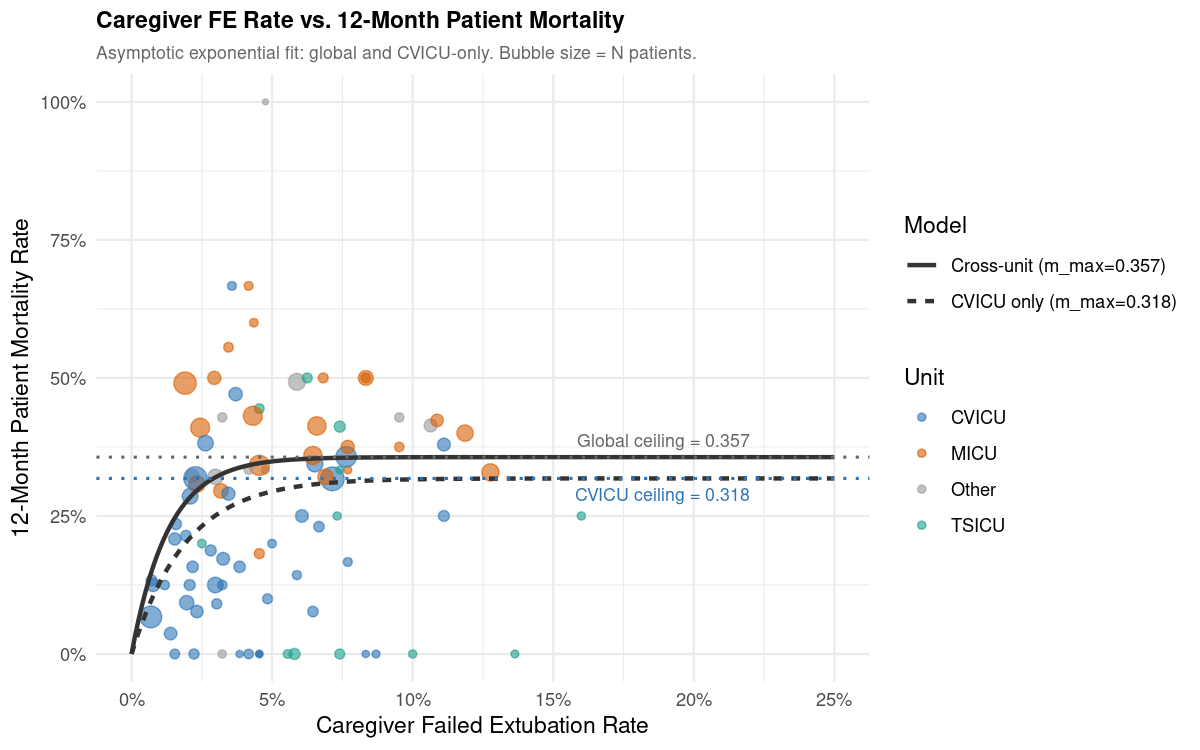
\includegraphics[width=0.8\textwidth]{../figures/nls_stratified.png}
\caption{Caregiver FE rate vs.\ 12-month mortality at the caregiver level.
Asymptotic exponential fits: global (cross-unit, $N=90$) and CVICU-only
($N=44$). Mortality ceiling $m_{\max}$ = 0.357 globally, 0.318 for CVICU.}
\label{fig:mortality_ceiling}
\end{figure}

%% ───────────────────────────────────────────────────
\section{Mixed effects models}

\begin{center}
\begin{tabular}{lrrrr}
\toprule
Model & Estimate & 95\% CI & $p$ / P($>$0) \\
\midrule
glmmTMB (caregiver\_fe\_rate, log-odds) & $+0.460$ & -- & $p = 0.660$ \\
rstanarm (caregiver\_fe\_scaled, posterior) & $+0.017$ & ($-0.071$, $0.103$) & 64.6\% \\
\bottomrule
\end{tabular}
\end{center}

\noindent Random effect variances: caregiver\_id $\approx 0$ (both models);
first\_careunit = 0.295 (glmmTMB), posterior mean 0.501 (rstanarm). The
unit-level random effect absorbs mortality differences across units, leaving
the caregiver FE rate fixed effect with no global signal to explain. This is
consistent with all other analyses showing the signal (to the extent it
exists) is CVICU-specific, not global. The near-zero caregiver-level random
effect variance is also consistent with the low denominator $R^2$ values in
the MSM: patients are not systematically routed to high-FE caregivers based
on their covariates, and caregiver-level clustering explains little variance
in outcomes once unit is accounted for.

\section{Deep Learning Models}

A Python pipeline trains three models on the same patient-level covariates
used in the R analyses (70/15/15 train/val/test split, seed 237): L2-regularized
logistic regression, gradient-boosted trees (GBM), and a multilayer perceptron
(MLP) with entity embeddings for ICU unit, intubation type, primary diagnosis,
and sex. These are predictive benchmarks, not causal models. They ask whether
flexible nonlinear interactions improve discrimination and whether caregiver FE
rate contributes to prediction once the network can exploit richer feature
interactions.

\subsection{Predictive performance}

\begin{center}
\begin{tabular}{lrrr}
\toprule
Model & AUC-ROC & AUC-PR & Brier \\
\midrule
Logistic regression (test) & 0.829 & 0.663 & 0.149 \\
Gradient boosting (test)   & 0.852 & 0.674 & 0.141 \\
MLP (test, best ep.\ 16)   & 0.841 & 0.670 & 0.166 \\
\bottomrule
\end{tabular}
\end{center}

\noindent The MLP matches gradient boosting closely (test AUC 0.841 vs.\ 0.852
at early-stopping epoch 16), indicating no deep nonlinear structure beyond what
the tree ensemble already captures at this sample size ($N = 3{,}437$).
All models substantially outperform the mortality-rate baseline
(AUC-PR $\approx 0.30$ for a random classifier at 30\% prevalence), consistent
with the R regression models showing that SOFA, Charlson, and ICU unit predict
outcomes well.

\subsection{SHAP feature importance}

\begin{figure}[h!]
\centering
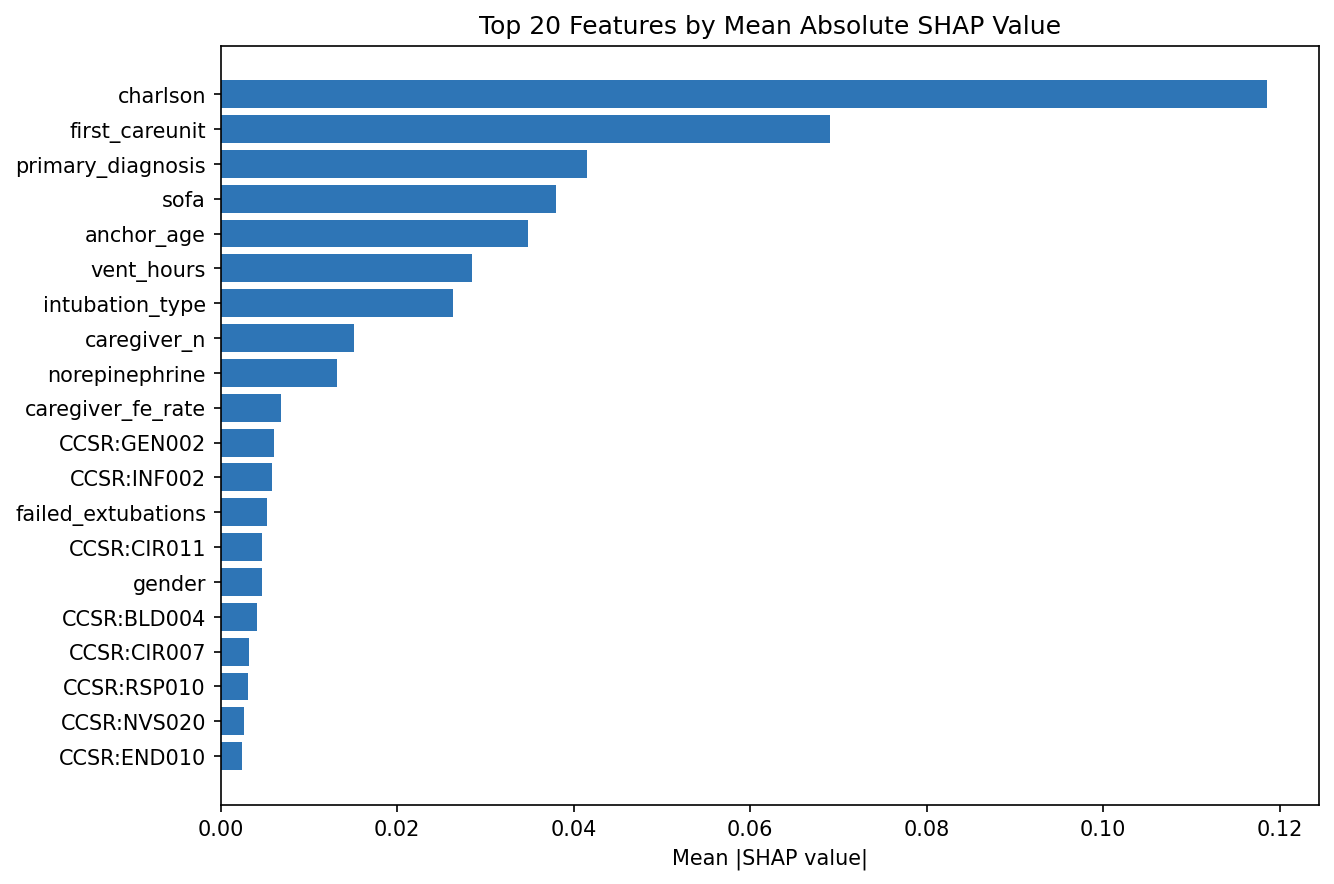
\includegraphics[width=0.75\textwidth]{../python/figures/shap_bar.png}
\caption{Top 20 features by mean $|$SHAP value$|$ from the MLP (200 test-set
patients, KernelExplainer). Features are ordered by global importance.}
\label{fig:shap_bar}
\end{figure}

The SHAP ranking (Figure~\ref{fig:shap_bar}) is consistent with the R
analyses. Charlson comorbidity index is the dominant predictor by a wide
margin; SOFA ranks second and \texttt{first\_careunit} (ICU unit embedding)
ranks third --- confirming that illness severity and unit-level case-mix
differences are the primary drivers of mortality heterogeneity. Ventilation
hours, primary diagnosis, and age follow. Caregiver FE rate ranks 8th out of
36 features, with a positive direction in the SHAP dependence plot (higher FE
rate pushes predicted mortality upward), consistent with all R analyses. Its
modest rank relative to Charlson and unit reflects the same finding as the
mixed-effects and MSM models: FE rate carries directionally consistent signal
within units but is dominated globally by patient severity and case-mix.

\subsection{Double/Debiased ML (DML)}
\label{sec:dml}

The partially linear DML estimator (Chernozhukov et al.\ 2018) uses 5-fold
cross-fitting with GBM nuisance models to partial out all measured confounders
from both the outcome and the treatment, then estimates $\hat{\theta}$ by
regressing the mortality residual on the FE rate residual. The estimand is
$\Delta P(\text{mortality})$ per unit of FE rate. The analysis has been
rerun on the updated cohort (\texttt{caregiver\_unit\_n} $\geq 20$, outcome =
12-month mortality as defined in the Python pipeline; see note below on
the mortality definition) stratified by ICU group, matching the R MSM
analysis.

\begin{table}[h!]
\centering
\begin{tabular}{lrrrrr}
\toprule
Group & N & $\hat{\theta}$ & 95\% CI & $p$ & IQR effect \\
\midrule
CVICU           & 1,435 & $+1.062$ & $[-0.550,\,+2.673]$ & 0.197 & $+2.3$ pp \\
Medical         & 1,001 & $-0.542$ & $[-1.980,\,+0.896]$ & 0.460 & $-2.2$ pp \\
Surgical/Trauma &   809 & $-0.696$ & $[-2.163,\,+0.771]$ & 0.352 & $-2.2$ pp \\
\midrule
Global (\texttt{explicit\_extubations}) & 3,437 & $-0.333$ & $[-1.010,\,+0.344]$ & 0.335 & $-1.4$ pp \\
\bottomrule
\end{tabular}
\caption{DML results. Unit-stratified rows use \texttt{caregiver\_unit\_n} $\geq 20$
($N = 3{,}245$ primary-group patients). Global row uses \texttt{explicit\_extubations}
($N = 3{,}437$; \texttt{caregiver\_n} $\geq 20$, all units). IQR effect =
$\hat{\theta} \times$ IQR of \texttt{caregiver\_fe\_rate} within the group.
All estimates are null. CVICU is directionally positive (higher FE rate
$\to$ higher mortality), consistent with the MSM and the caregiver-level
partial correlation. Medical, Surgical/Trauma, and Global are
directionally negative but also null.
Overall cohort mortality rate 30.1\% matches the R analysis.}
\label{tab:dml}
\end{table}

\begin{figure}[h!]
\centering
\includegraphics[width=0.80\textwidth]{../python/figures/dml_cvicu.png}
\caption{DML partialled-out scatter (left) and FE rate residual distribution
(right) for CVICU. $\hat{\theta} = +1.062$, $p = 0.197$. The wide confidence
interval reflects both the small IQR of FE rate in CVICU (2.1 pp) and the
limited residual variation in FE rate after GBM partialling.}
\label{fig:dml_cvicu}
\end{figure}

\noindent \textbf{Treatment R$^2$ interpretation.} The GBM treatment model
achieves R$^2 \approx 0.53$--$0.69$ for the unit-stratified models and
R$^2 \approx 0.52$--$0.60$ globally, substantially higher than the
linear OLS denominator R$^2 = 0.057$ from the R MSM. The GBM is capturing
nonlinear or interaction-based patterns in FE rate that OLS misses. The most
likely explanation is caregiver-level clustering: patients of the same
caregiver share the same FE rate, and patient profiles are weakly correlated
with caregiver identity in ways a GBM can exploit. Despite this higher
treatment predictability, all $\hat{\theta}$ estimates are null --- confirming
that even the additional variation the GBM explains does not translate to a
causal FE rate effect on mortality.

\noindent All three groups are null. CVICU is directionally positive
($\hat{\theta} = +1.062$, IQR effect +2.3 pp, $p = 0.197$), consistent
with the MSM and the caregiver-level partial correlation. Over the CVICU
FE rate IQR of 2.1 pp, the implied mortality difference is just 2.3 pp ---
small and well within the confidence interval. Medical and Surgical/Trauma
are directionally negative but also null ($p = 0.46$, $0.35$). The wide
confidence intervals in all groups reflect the limited residual FE rate
variation after the GBM has removed patient-level confounding (treatment
$R^2 \approx 0.53$--$0.69$), confirming that the causal signal, if it
exists, is smaller than what these data can resolve.


\section{Trajectory Analysis}
\label{sec:trajectory}

Andrew's proposed dynamic risk framework requires that reintubation risk
be estimable as a function of time on the ventilator, so that the optimal
extubation time can be identified as the point where one more day of waiting
produces less than approximately 0.5\% reduction in failure probability.
We tested whether two standard readiness variables --- RSBI and P/F ratio
--- carry the trajectory information this framework requires.

\subsection{Data}

RSBI (spontaneous respiratory rate / spontaneous tidal volume in liters)
and P/F ratio (PaO$_2$/FiO$_2$) were pulled from MIMIC-IV for all explicit
extubation events in the \texttt{all\_extubations} cohort (6,063 events,
5,505 patients). The outcome is \texttt{failed\_extubation\_flag}: reintubation
within 72 hours of this specific extubation event. This is the per-event
outcome, not the patient-lifetime reintubation count.

\begin{center}
\begin{tabular}{lrr}
\toprule
Variable & Events with $\geq$3 measurements & Failed extubations \\
\midrule
RSBI & 3,551 & 395 (11.1\%) \\
P/F ratio & 3,747 & 345 (9.2\%) \\
\bottomrule
\end{tabular}
\end{center}

\subsection{Individual-level slope analysis}

For each extubation event with $\geq$3 measurements in the 72h window,
a linear slope was estimated by fitting \texttt{lm(measurement \textasciitilde{}
hours\_before\_extubation)}. A negative slope indicates the variable is
improving as extubation approaches.

\begin{center}
\begin{tabular}{lrrrr}
\toprule
 & \multicolumn{2}{c}{Succeeded} & \multicolumn{2}{c}{Failed} \\
 & Mean slope & Mean at extub & Mean slope & Mean at extub \\
\midrule
RSBI & $-0.782$ & 48.7 & $-0.290$ & 52.3 \\
P/F ratio & $-0.627$ & 256 & $-0.272$ & 251 \\
\bottomrule
\end{tabular}
\end{center}

\noindent Both variables show slopes in the expected direction --- succeeded
events have more steeply declining (improving) trajectories --- but the
difference is small relative to within-patient noise.

Logistic regression testing whether slope predicts failure beyond level at
extubation:

\begin{center}
\begin{tabular}{lrrrr}
\toprule
Predictor & Coefficient & SE & $z$ & $p$ \\
\midrule
\textit{RSBI model:} & & & & \\
\quad Level at extubation & 0.0032 & 0.0015 & 2.14 & 0.032 \\
\quad Slope (72h window) & 0.0017 & 0.0036 & 0.48 & 0.634 \\
\addlinespace
\textit{P/F ratio model:} & & & & \\
\quad Level at extubation & $-0.0004$ & 0.0006 & $-0.67$ & 0.505 \\
\quad Slope (72h window) & 0.0015 & 0.0044 & 0.35 & 0.726 \\
\bottomrule
\end{tabular}
\end{center}

\noindent RSBI level at extubation is a significant predictor ($p = 0.032$);
neither slope is significant ($p = 0.634$ and $p = 0.726$). The trajectory
of RSBI or P/F ratio in the 72 hours before extubation carries no independent
predictive information beyond the level at the moment of extubation.

\subsection{Population-level trajectories}

Figure~\ref{fig:trajectories} shows hourly mean RSBI and P/F ratio in the
72h before extubation, split by outcome.

\begin{figure}[h!]
\centering
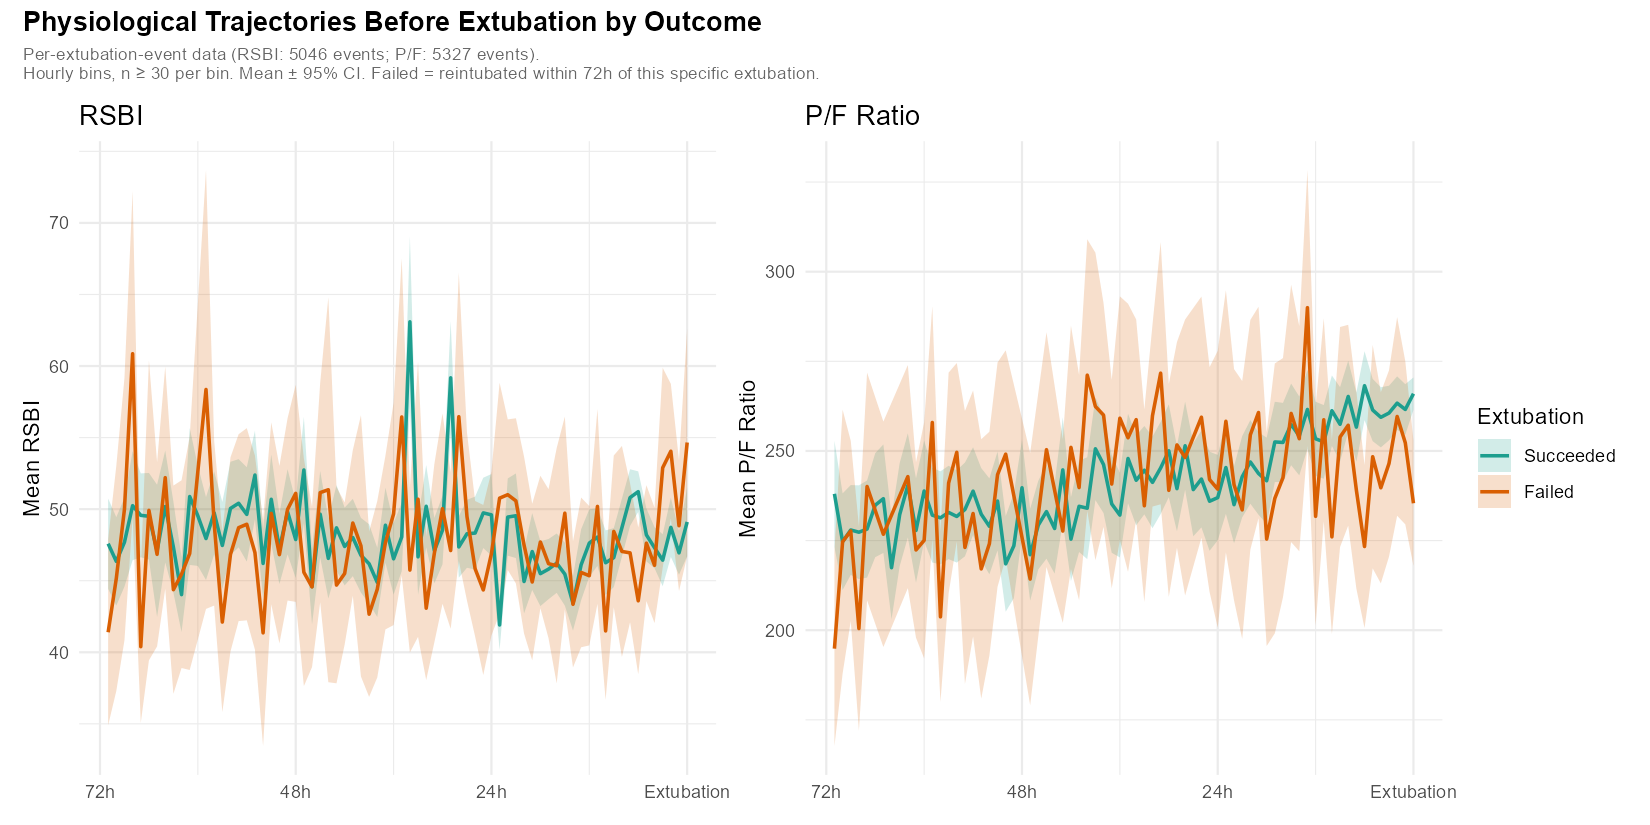
\includegraphics[width=0.95\textwidth]{../figures/preextubation_trajectories_by_event_outcome.png}
\caption{RSBI and P/F ratio in the 72h before extubation by outcome (failed
vs.\ succeeded). Hourly bins, $n \geq 30$ per bin, mean $\pm$ 95\% CI.
The two groups are largely indistinguishable throughout the window. The
zigzag in the failed group reflects genuine measurement noise with
approximately 400 failed events distributed across 72 hourly bins.}
\label{fig:trajectories}
\end{figure}

\subsection{Interpretation}

The null slope finding is consistent with two non-exclusive explanations.
First, RSBI and P/F ratio may not be sensitive enough variables to detect
the trajectory signal --- they are measured infrequently (median 4--6
measurements per patient in the 72h window) and are inherently noisy.
Second, clinicians may already be conditioning on trajectory implicitly ---
extubating only after the patient has plateaued at a low RSBI --- so that
by the time of extubation the trajectory information is spent.

The dynamic risk framework remains theoretically sound. Implementing it
prospectively would require variables with higher temporal resolution than
are available in retrospective EHR data: continuous pressure support level,
FiO$_2$ weaning trajectory, and spontaneous breathing trial (SBT) outcomes
are candidates. Retrospective validation from MIMIC-IV data alone is not
feasible with current measurement density.

\begin{todo}
\textbf{TODO --- SBT outcomes:} Spontaneous breathing trial pass/fail
is documented in MIMIC-IV chartevents. Whether SBT outcome predicts
extubation failure beyond RSBI level is a direct test of the dynamic
risk hypothesis and is feasible with existing data.
\end{todo}

%% ─────────────────────────────────────────────────────────────────────────────
\section{Limitations}

\begin{enumerate}[leftmargin=*]

\item \textbf{Caregiver attribution.} \texttt{caregiver\_id} records the
documenting user, not necessarily the provider who performed the extubation.
This introduces measurement error in the exposure variable that would tend to
attenuate any real signal toward the null.

\item \textbf{Case mix confounding within CVICU.} The volume confounding
analysis demonstrates that 0\%-FE-rate caregivers systematically see shorter,
simpler cases. Even with \texttt{caregiver\_unit\_n} $\geq 20$, residual case mix
differences that are not captured by the measured covariates may explain the
partial correlation ($r = +0.261$) seen at the caregiver level. The null
causal estimates across methods (MSM OR = 1.432, $p = 0.102$; DML
$\hat{\theta} = +1.062$, $p = 0.197$) are the strongest evidence that this
association does not reflect a causal effect once patient-level confounders
are removed.

\item \textbf{Single center.} MIMIC-IV is from Beth Israel Deaconess Medical
Center. An eICU parallel analysis (208 ICUs, with possible caregiver type
information) is planned to assess generalizability.

\item \textbf{Caregiver type unknown.} Whether \texttt{caregiver\_id}
corresponds to an attending physician, APP, or trainee is not directly
available in MIMIC-IV. Andrew asks whether this information exists; it may
be recoverable via the \texttt{caregivers} table, which requires a targeted
BigQuery query.

\item \textbf{Terminal extubation misclassification.} The 3-day mortality
criterion captures some patients extubated with survival intent who
deteriorated unexpectedly. A code status change marker would be more specific
(planned; see Section~\ref{sec:terminal}).

\item \textbf{All-cause 12-month mortality.} Deaths unrelated to the index
extubation are counted. Shorter-term outcomes (hospital and 30-day mortality)
are consistent in direction with the 12-month endpoint.

\item \textbf{Missed extubation opportunities.} Patients extubated too late
cannot be identified in retrospective data without knowing the counterfactual.
This is the motivation for the dynamic risk analysis (Section~\ref{sec:trajectory}).

\end{enumerate}

%% ─────────────────────────────────────────────────────────────────────────────
\section{Proposed Next Steps}

\begin{enumerate}[leftmargin=*]

\item \textbf{Code status query (BigQuery).} Pull DNR/DNI orders from
MIMIC-IV \texttt{chartevents} and identify code status changes in the 24--48h
before extubation. This provides a more specific terminal extubation marker
than the 3-day mortality proxy.

\item \textbf{CONSORT diagram.} Cohort flow figure (script 09\_consort.R)
for the paper.

\item \textbf{SBT outcomes analysis.} Spontaneous breathing trial pass/fail
documented in MIMIC-IV chartevents (see Section~\ref{sec:trajectory}).

\item \textbf{eICU exploratory analysis.} 208 ICUs, potential caregiver type
information, external validation of CVICU partial correlation finding.

\item \textbf{Citation manager.} Zotero recommended.

\end{enumerate}

\end{document}
